\documentclass[11pt,aspectratio=169]{beamer}
\usetheme{metropolis}
\usepackage{amsmath,amssymb,booktabs}
\usepackage[T1]{fontenc}
\usepackage{graphicx}
\usepackage{xcolor}

\definecolor{ink}{HTML}{0B0B0B}
\definecolor{ink2}{HTML}{52514E}
\definecolor{blu}{HTML}{2A78D6}
\definecolor{org}{HTML}{EB6834}
\definecolor{aqu}{HTML}{1BAF7A}
\definecolor{surf}{HTML}{FCFCFB}
\setbeamercolor{normal text}{fg=ink,bg=surf}
\setbeamercolor{frametitle}{fg=surf,bg=ink}
\setbeamercolor{alerted text}{fg=org}
\setbeamercolor{progress bar}{fg=aqu,bg=black!12}
\metroset{sectionpage=progressbar,numbering=fraction,block=fill}
\setbeamerfont{frametitle}{size=\large}
\setbeamertemplate{itemize items}[square]
\setbeamercolor{itemize item}{fg=aqu}
\setbeamercolor{itemize subitem}{fg=ink2}

\newcommand{\tk}[1]{{\color{ink2}\footnotesize #1}}
\newcommand{\rs}{$r^{*}$}

\title{The FOMC Window}
\subtitle{What is identified, what is not, and where the project goes next}
\date{11 August 2026}
\author{Progress report}

\begin{document}

\maketitle

% =====================================================================
\section{The motivating fact}

\begin{frame}{Long rates fall only when the Fed is in the room}
\begin{center}
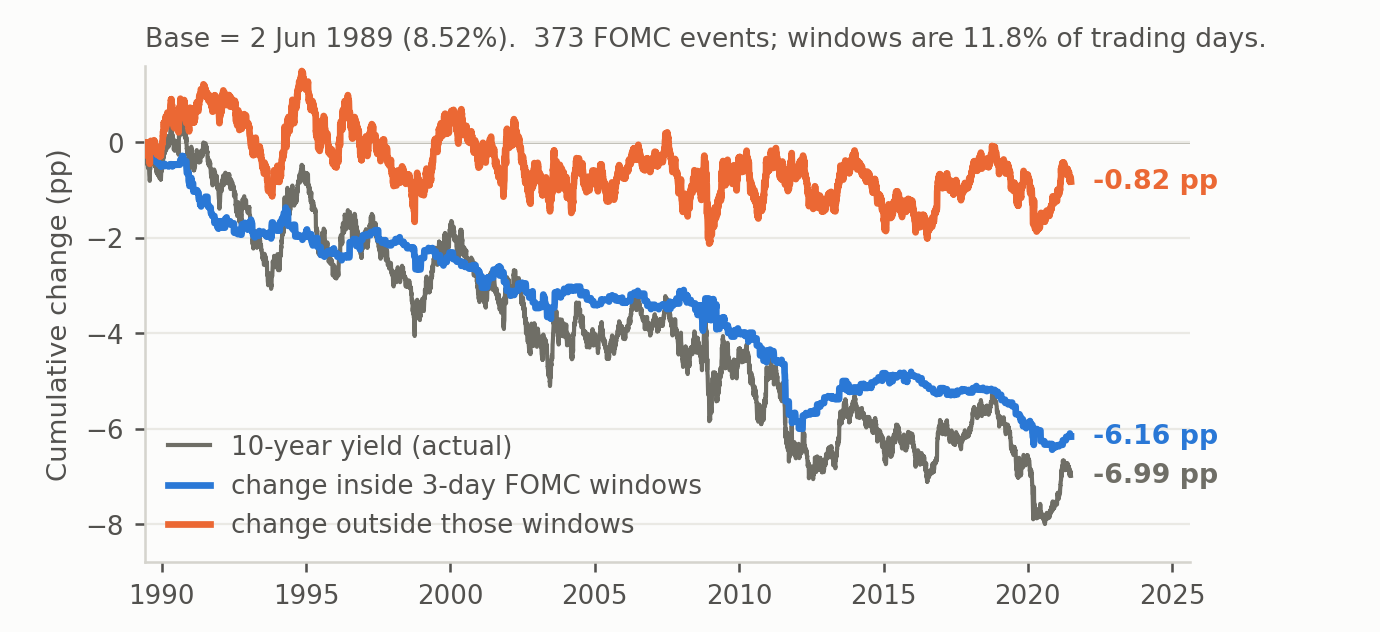
\includegraphics[width=0.88\linewidth]{s_fact.png}
\end{center}
\vspace{-0.5em}
\tk{Hillenbrand (2025, \emph{RFS}), replicated from GSW yields and a hand-built FOMC calendar.}
\end{frame}

\begin{frame}{The fact is really an absence}
\begin{columns}[T]
\begin{column}{0.52\textwidth}\small
\begin{itemize}\setlength\itemsep{0.25em}
  \item Three-day windows are \alert{11.8\%} of trading days but carry \alert{88\%} of a 6.99 pp decline.
  \item The per-meeting effect is small: $-2.5$ bp.
  \item What is remarkable is the other 88\% of days: drift of $-0.012$ bp/day, $t=-0.18$, over 7{,}035 days.
  \item Randomisation test: 324 randomly placed 3-day blocks on non-FOMC days, 5{,}000 draws. Observed $-6.16$ pp sits at the 0th percentile, $p<0.0002$.
\end{itemize}
\end{column}
\begin{column}{0.46\textwidth}
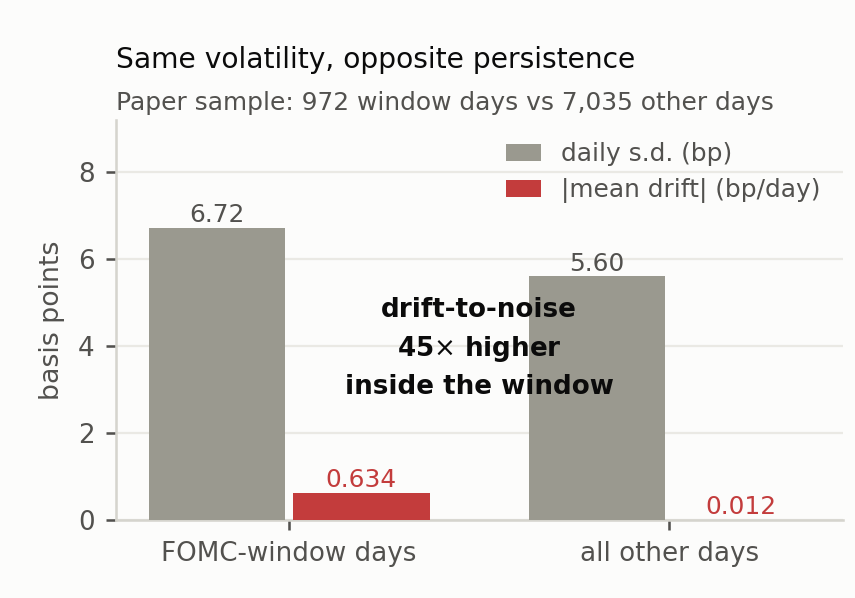
\includegraphics[width=\linewidth]{s_persist.png}
\end{column}
\end{columns}
\end{frame}

\begin{frame}{The question this raises}
\begin{block}{Motivation}
If the Fed sets an overnight rate, why does the \emph{ten-year} rate move only on its calendar --- and why do those moves not wash out?
\end{block}
\vspace{0.3em}
\begin{block}{The question I set out to answer}
When the Fed moves long rates at scheduled announcements, is it changing \alert{where markets think rates are going} (expected short rates), or \alert{what markets charge for the risk of being wrong} (the term premium)?
\end{block}
\vspace{0.3em}
\tk{Accounting identity behind it:\quad $y^{(n)}_t = r^{*}_t + \pi^{*}_t + \tfrac1n\sum_j E_t[\text{gap}_{t+j}] + TP^{(n)}_t$}
\vspace{0.2em}

\tk{With the inflation target fixed, ``the Fed moves long rates'' is close to ``the Fed moves beliefs about \rs{}'' --- which is why \rs{} became central to the project. The next slide says how close.}
\end{frame}

\begin{frame}{What exactly is the ``gap''?}
\small
Define the neutral nominal rate $i^{*}_t\equiv r^{*}_t+\pi^{*}_t$ and the \emph{policy gap}
$\text{gap}_t\equiv i_t-i^{*}_t$ --- the stance of policy. Under a Taylor rule,
$\text{gap}_t=\phi_\pi(\pi_t-\pi^{*}_t)+\phi_x x_t+v_t$: cyclical and mean-reverting.
\vspace{0.2em}

If it decays as an AR(1) with monthly persistence $\rho$, then
$\frac1n\sum_j E_t[\text{gap}_{t+j}]=\omega(\rho,n)\,\text{gap}_t$ with
$\omega=\dfrac{1-\rho^{n}}{n(1-\rho)}$ --- \alert{small, but not zero}:
\vspace{-0.2em}
\begin{center}\footnotesize
\begin{tabular}{lccc}
\toprule
Half-life of the gap & $\omega$, 2y & $\omega$, 5y & $\omega$, 10y\\ \midrule
1 year & 0.56 & 0.29 & 0.15\\
2 years & 0.73 & 0.48 & 0.28\\
4 years & 0.85 & 0.67 & 0.48\\
\bottomrule\end{tabular}
\end{center}
\vspace{-0.4em}
\footnotesize
Over an announcement window,
\vspace{-0.6em}
\[
\Delta y^{(n)}_t=\underbrace{\Delta r^{*}_t+\Delta\pi^{*}_t}_{\text{endpoint news}}
+\underbrace{\omega\,\Delta\text{gap}_t+\text{gap}_t\,\Delta\omega}_{\text{stance and persistence news}}
+\Delta TP^{(n)}_t .
\]
\vspace{-0.5em}
\alert{Four terms, one observable} --- and $\pi^{*}$ is only plausibly fixed after $\sim$2000.
\end{frame}

% =====================================================================
\section{What the literature has established}

\begin{frame}{The core fact and its extensions}
\footnotesize
\begin{tabular}{@{}p{0.30\textwidth}p{0.62\textwidth}@{}}
\toprule
\textbf{Paper} & \textbf{What it establishes}\\ \midrule
Hillenbrand (2025, \emph{RFS}) & The whole secular decline in the 10-year accumulates in 3-day FOMC windows, 1989--2021. Attributes it to markets learning a lower \rs{} from the Fed.\\[0.35em]
Hofmann, Li \& Wu (BIS 1252) & The pattern is global --- 10 advanced economies --- and survives a shifting-endpoint model.\\[0.35em]
Hanson, Lucca \& Wright (2021, \emph{QJE}) & Announcement-window long-rate moves \emph{substantially reverse} within 6--12 months. Read as evidence of temporary term-premium effects.\\[0.35em]
Bauer \& Swanson (2023, \emph{NBER MA}) & Announcement surprises are predictable from pre-meeting public data; the ``Fed information effect'' is largely the Fed responding to news.\\
\bottomrule
\end{tabular}
\vspace{0.4em}

\tk{Rows 1 and 3 are in tension: Hillenbrand's fact requires window moves \emph{not} to reverse.}
\end{frame}

\begin{frame}{The contested channel}
\footnotesize
\begin{tabular}{@{}p{0.30\textwidth}p{0.62\textwidth}@{}}
\toprule
\textbf{Paper} & \textbf{What it establishes}\\ \midrule
Hofmann, Li \& Wu (BIS 1252) & The window decline is \alert{risk-neutral} (US pseudo-$R^2$ 96 vs 32). \tk{But the endpoint is defined as PC1 of cumulative FOMC-window yield changes --- it inherits the series being explained.}\\[0.35em]
Pan \& Peng (SSRN 4764451) & On day $t-1$ the decline is \alert{term premium}: $-0.71$ of $-0.79$ bp; expectations $-0.08$, insignificant.\\[0.35em]
Joslin, Singleton \& Zhu (2011); Joslin, Priebsch \& Singleton (2014) & Under spanning the state is recoverable from yields, so the expectations component is a fixed linear function of the curve.\\[0.35em]
Bauer \& Rudebusch (2020, \emph{AER}); (2014, \emph{IJCB}) & A stationary VAR books genuine endpoint shifts as term premium: 75\% vs 35--37\% for the secular decline.\\
\bottomrule
\end{tabular}
\vspace{0.4em}

\tk{Two papers, opposite answers, neither adjudicated.}
\end{frame}

\begin{frame}{The beliefs-about-\rs{} strand}
\footnotesize
\begin{tabular}{@{}p{0.30\textwidth}p{0.62\textwidth}@{}}
\toprule
\textbf{Paper} & \textbf{What it establishes}\\ \midrule
Bauer, Pflueger \& Sunderam (2024, \emph{QJE}) & A pre-meeting \emph{subjective belief} --- the perceived policy reaction-function \emph{slope} --- is related to term premia and to state-dependent window responses. The template for this design.\\[0.35em]
Ahonon \& Roussellet (FRBNY SR 1187) & Under learning about unobserved trends, investor uncertainty about \rs{} is $\pm$170 bp, not $\pm$55 bp; \rs{} is the primary long-run driver of bond risk premia.\\[0.35em]
Couture (2021); Engstrom (FEDS 2026-026) & The dot plot moves asset prices; SEP-minus-market gaps predict forecast errors.\\[0.35em]
Favero, Melone \& Tamoni (2024, \emph{JFQA}) & A policy-rate-minus-equilibrium-rate gap predicts bond returns. \tk{Different wedge, similar name --- must be differentiated explicitly.}\\
\bottomrule
\end{tabular}
\vspace{0.3em}

\tk{Never tested: the perceived \emph{endpoint} --- not how strongly markets think the Fed responds, but where they think it is heading.}
\end{frame}

% =====================================================================
\section{What our extensions add}

\begin{frame}{Extension 1: the event list decides the answer}
\begin{center}
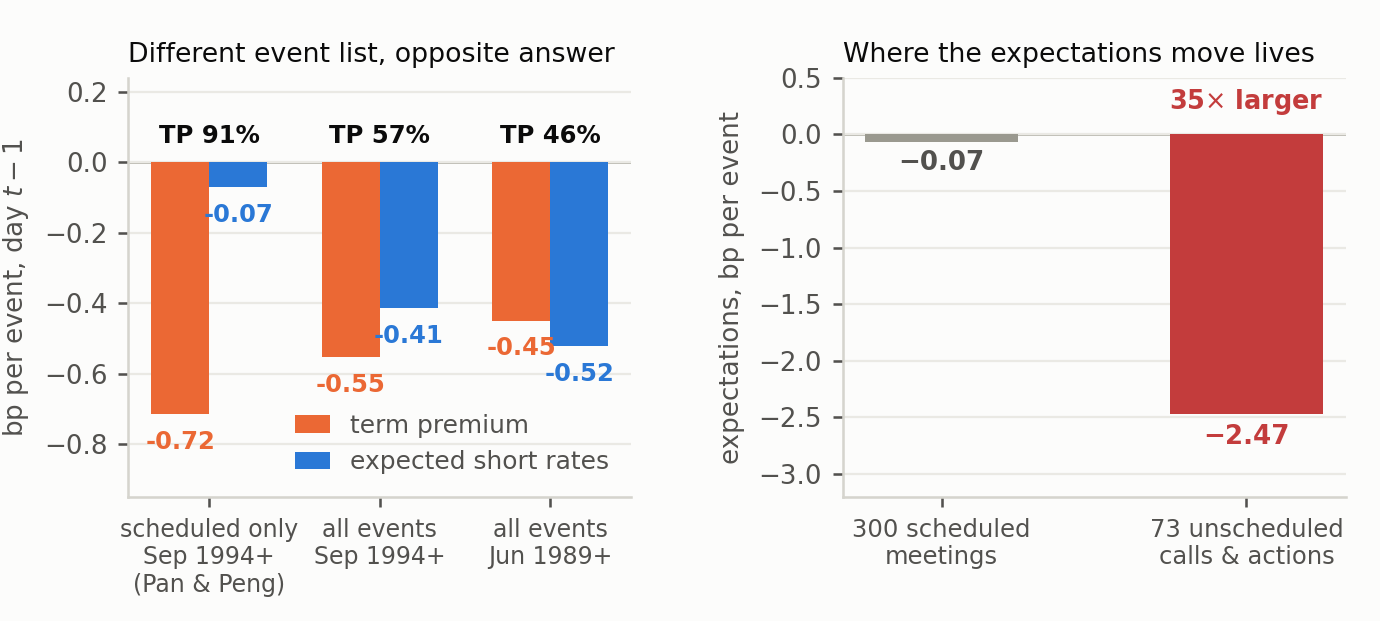
\includegraphics[width=0.70\linewidth]{s_eventlist.png}
\end{center}
\vspace{-0.5em}
\scriptsize
\begin{itemize}\setlength\itemsep{0.15em}
  \item Pan \& Peng replicated to three coefficients ($-0.785$ / $-0.716$ / $-0.070$). Their filter --- scheduled meetings only, 1994+ --- \alert{drops 73 calls and intermeeting actions}.
  \item Same day, same data, same decomposition: the term-premium share moves \alert{91\% $\rightarrow$ 46\%}.
  \item \textbf{New:} the two contradictory papers are reconciled without taking a side on the model.
\end{itemize}
\end{frame}

\begin{frame}{Extension 2: the sample through July 2026}
\begin{center}
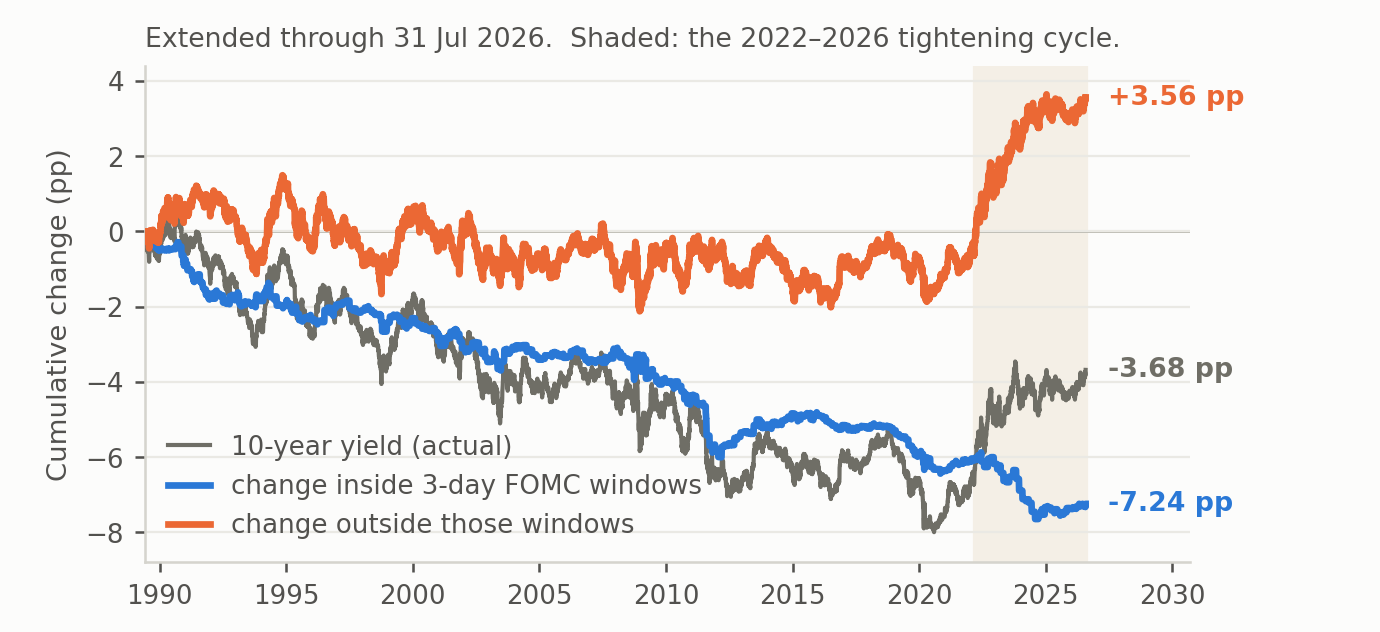
\includegraphics[width=0.70\linewidth]{s_extend.png}
\end{center}
\vspace{-0.5em}
\scriptsize
\begin{itemize}\setlength\itemsep{0.15em}
  \item 2022--2026: the Fed raised the target 525 bp and the 10-year rose 2.60 pp. \alert{In windows it \emph{fell} 1.20 pp --- the entire increase happened outside.}
  \item The in-window series keeps declining, to $-7.24$ pp, straight through the tightening.
  \item \textbf{New:} no paper covers this period, and the pattern is not symmetric in the direction of policy.
\end{itemize}
\end{frame}

\begin{frame}{Extension 3: the decomposition cannot arbitrate}
\begin{center}
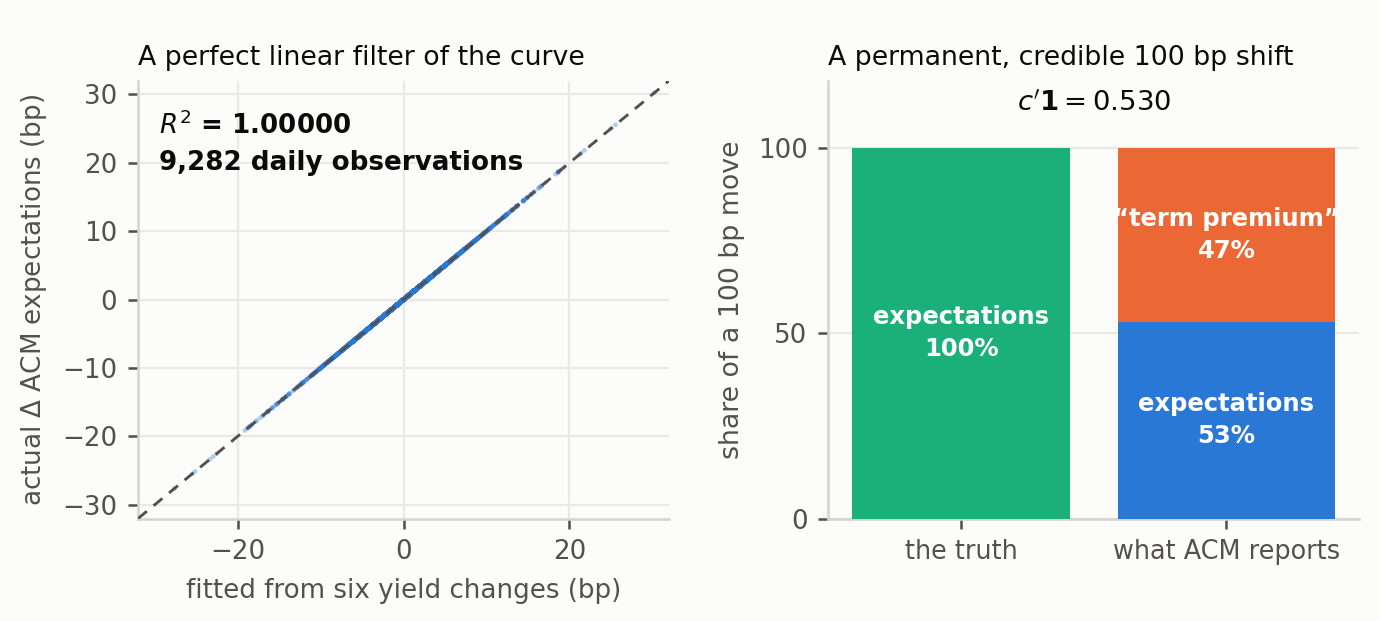
\includegraphics[width=0.70\linewidth]{s_acmfilter.png}
\end{center}
\vspace{-0.5em}
\scriptsize
\begin{itemize}\setlength\itemsep{0.15em}
  \item $\Delta rn^{(n)}_t=c_n'\Delta y^{\mathcal N}_t$, $c_n'=b_n'\mathbf B^{-1}$; empirically $R^2=1.00000$, so $\beta^{rn}=c'\beta^{\mathcal N}$ (predicted $+2.5$/$+29.3$ vs estimated $+2.6$/$+29.2$ bp).
  \item \alert{The decomposition adds no event-specific information}, and $c'\mathbf 1=0.529$ mis-books half of a permanent credible shift.
  \item \textbf{Attribution:} algebra from JSZ (2011), bias from Bauer--Rudebusch; mine is the ACM filter and the event-study corollary.
\end{itemize}
\end{frame}

% =====================================================================
\section{Where \rs{} enters}

\begin{frame}{Why \rs{} is the natural mechanism --- and the natural test}
\begin{block}{The logic}
The Fed's 2\% target is fixed and credible, so a permanent move in the 10-year that is \emph{not} a risk premium has to be a move in beliefs about the real endpoint. ``The Fed moves long rates'' $\Rightarrow$ ``the Fed moves beliefs about \rs{}.''
\end{block}
\vspace{0.2em}
\begin{block}{The design it suggested}
Does the pre-meeting gap between the \alert{Fed's published longer-run projection} and the \alert{market-implied endpoint} predict the window response --- and does it load on the term premium or on expectations?
\end{block}
\vspace{0.3em}
\begin{itemize}
  \item Needs a Fed leg: the SEP longer-run dot, available from 2012.
  \item Needs a market leg: an endpoint measure \emph{not} built from FOMC-window data.
\end{itemize}
\end{frame}

\begin{frame}{The treatment exists; the control does not}
\begin{center}
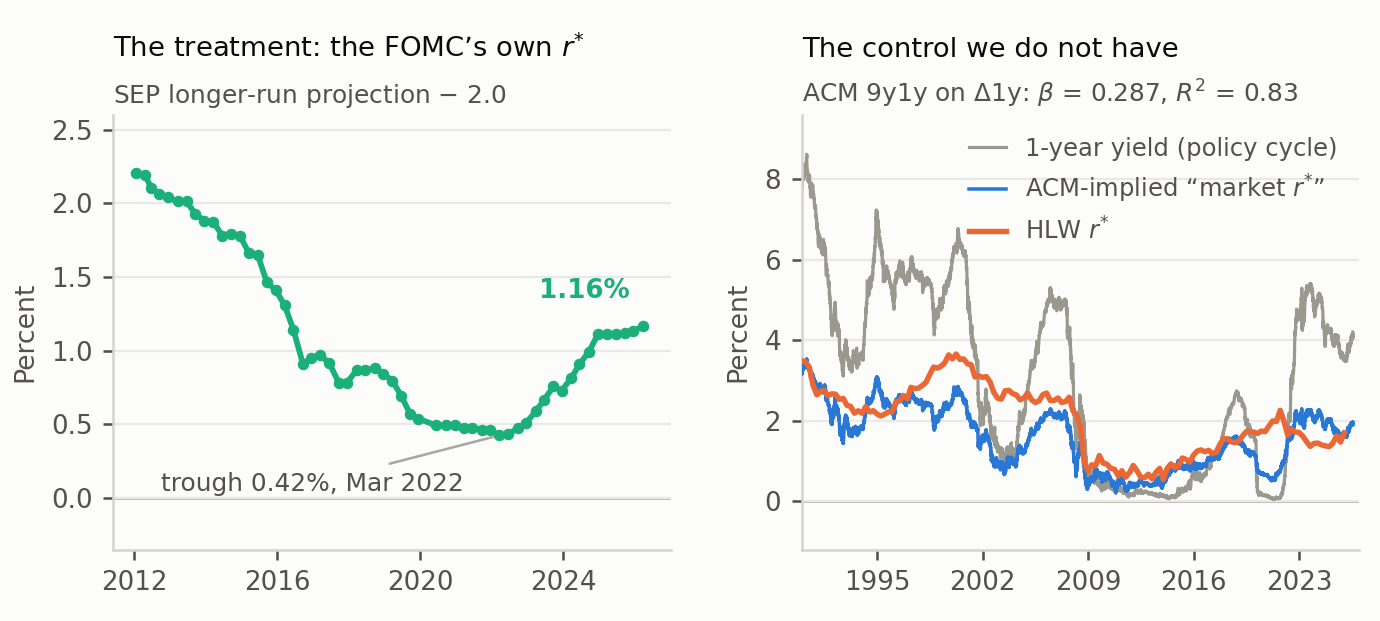
\includegraphics[width=0.70\linewidth]{s_rstar.png}
\end{center}
\vspace{-0.5em}
\scriptsize
\begin{itemize}\setlength\itemsep{0.15em}
  \item The Fed leg is real and moves: $-1.78$ pp to Mar 2022, then $+0.74$ pp; 48 distinct values in the mean dot.
  \item The market leg fails --- the ACM 9y1y forward is \alert{a damped copy of the policy cycle} ($\beta=0.287$, $R^2=0.83$, level corr.\ $+0.984$).
  \item Structural, not a bad horizon choice: under a stationary VAR $b_n\!\to\!0$, so \emph{no} horizon isolates an endpoint. Survey alternatives correlate $-0.12$ with it.
\end{itemize}
\end{frame}

\begin{frame}{And the treatment window is the wrong decade}
\begin{center}
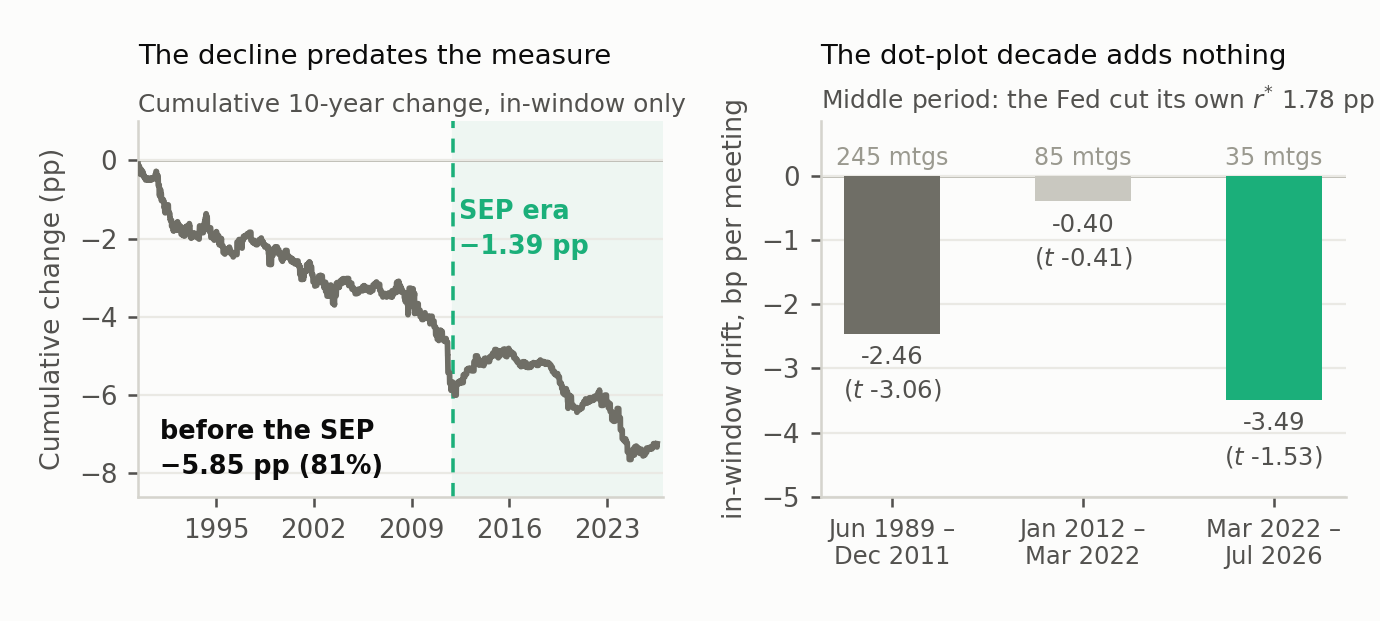
\includegraphics[width=0.70\linewidth]{s_timing.png}
\end{center}
\vspace{-0.5em}
\scriptsize
\begin{itemize}\setlength\itemsep{0.15em}
  \item \alert{81\% of the in-window decline is complete before the dot plot begins.}
  \item In the decade when the Fed cut its own longer-run rate 1.78 pp --- when an information channel should be loudest --- the in-window drift is $-0.40$ bp/meeting, $t=-0.41$.
  \item Every projection-based test of this channel, the published one included, is run where there is almost nothing left to explain.
\end{itemize}
\end{frame}

% =====================================================================
\section{Preliminary results and next steps}

\begin{frame}{What survives}
\footnotesize
\begin{tabular}{@{}p{0.28\textwidth}p{0.34\textwidth}p{0.28\textwidth}@{}}
\toprule
\textbf{Result} & \textbf{Identifying assumption} & \textbf{Status}\\ \midrule
Event-list reconciliation: TP share 91\% $\to$ 46\% & None beyond the ACM series being the same object in both papers & Finished; most immediately publishable\\[0.25em]
ACM is a fixed filter, $R^2=1$, $c'\mathbf 1=0.529$ & Spanning; ACM's own estimated loadings & Finished; theorem standard, application new\\[0.25em]
Timing fact: 81\% pre-dates the SEP & Window assignment only & Finished; reframes the projection literature\\[0.25em]
2022--26: tightening occurs entirely outside windows & Window assignment only & Finished; no other paper covers it\\[0.25em]
Fed--market wedge design & Requires a non-circular market endpoint & \alert{Set aside} --- no such measure available\\
\bottomrule
\end{tabular}
\end{frame}

\begin{frame}{The unanswered question I would build on}
\begin{block}{The puzzle}
Window and non-window days have nearly identical daily volatility (6.72 vs 5.60 bp) but completely different cumulative outcomes ($-6.16$ vs $-0.82$ pp). Drift-to-noise is \alert{45$\times$} higher inside the window.
\end{block}
\vspace{0.2em}
So the question is not \emph{which component moves} --- it is
\begin{center}
\alert{\large why do only scheduled-date price changes persist?}
\end{center}
\vspace{0.1em}
\small
\begin{itemize}\setlength\itemsep{0.15em}
  \item A long-horizon variance-ratio decomposition by day type turns this from a description into a measured object.
  \item It needs no decomposition, no endpoint measure, and no model of the term premium --- so it survives every identification problem above.
  \item It confronts Hanson--Lucca--Wright (reversal) with Hillenbrand (permanence) directly.
\end{itemize}
\end{frame}

\begin{frame}{Path forward}
\small
\textbf{Immediate (four weeks)}
\begin{itemize}\setlength\itemsep{0.1em}
  \item[(a)] \textbf{Issuance test.} Lou, Pint\'er, \"Usl\"u \& Walker (BIS 1232) claim the effect concentrates in windows \emph{without} long-dated issuance. Auction dates are public; decisive either way in days.
  \item[(b)] \textbf{Draft the reconciliation note} (event list + timing fact). Self-contained and model-free.
\end{itemize}
\vspace{0.4em}
\textbf{Medium term (one term)}
\begin{itemize}
  \item[(c)] \textbf{Permanent vs transitory by day type} --- the variance-ratio design above. This is the chapter.
\end{itemize}
\vspace{0.4em}
\textbf{Contingent}
\begin{itemize}
  \item[(d)] \textbf{Extend the Fed-side measure back before 2012} using Tealbook/Greenbook projections (1981--2019, five-year lag) --- the only way to test any projection-based mechanism on the sample that contains the phenomenon.
\end{itemize}
\end{frame}

\begin{frame}{Where I would value guidance}
\begin{enumerate}\setlength\itemsep{0.5em}
  \item Is the reconciliation better as a standalone short submission, or folded into a chapter as a methodological section?
  \item Access to Blue Chip Financial Forecasts long-range and to the Tealbook archive --- both bind on (d).
  \item Is the permanent/transitory framing in (c) the right way to pose the question, or too descriptive to carry a chapter without a mechanism?
\end{enumerate}
\vspace{0.8em}
\tk{\textbf{Data.} G\"urkaynak--Sack--Wright zero-coupon yields; ACM daily decomposition, Jun 1989 -- Aug 2026; FOMC calendar built from Federal Reserve historical meeting pages (300 scheduled meetings plus 73 conference calls and unscheduled actions); SEP dot-plot archive, 57 meetings, Jan 2012 -- Mar 2026. All estimates recomputed from source.}
\end{frame}

\end{document}
